\documentclass[a4paper, czech]{article}

\usepackage[czech]{babel}
\usepackage{indentfirst}
\usepackage{graphicx}
\usepackage{float}
\usepackage[margin=1.5cm]{geometry}
\usepackage{booktabs}
\usepackage{amsmath}
\usepackage[table]{xcolor}
\usepackage{multirow}
\usepackage{tabularray}
\usepackage{bold-extra}


\begin{document}
\begin{table}[H]
    \centering
    \begin{tblr}{
        cell{1}{1} = {c = 2, r = 4}{c}, % Logo
        cell{1}{4} = {c = 3}{c}, % Předmět
        cell{2}{4} = {c = 3}{c}, % Jméno
        cell{3}{4} = {}{c}, % Ročník
        cell{3}{6} = {}{c}, % Studijní skupina
        cell{4}{4} = {}{c}, % Spolupracoval
        cell{4}{6} = {}{c}, % Mereno dne
        cell{5}{1} = {c = 2}{55mm}, % Kontroloval
        cell{5}{3} = {c = 2}{55mm}, % Hodnoceni
        cell{5}{5} = {c = 2}{55mm}, % Dne
        cell{6}{2} = {c = 5}{}, % Nazev ulohy
        cell{7}{1} = {}{c}, % Číslo úlohy
        cell{7}{2} = {c = 5}{c}, % Název úlohy
        vline{1,2,7} = {1.2pt},
        vline{3,5},
        hline{1,5,6,8} = {1.2pt},
        hline{2,3,4}
        }
        
\includegraphics{logo_fekt.png} & & \textsuperscript{Předmět} & \large \textbf{Měření v audiotechnice} \\
             & & \textsuperscript{Jméno} & \large \textbf{Karolína Šebestová} \\
             & & \textsuperscript{Ročník} & \large \textbf{3.} & \textsuperscript{Studijní skupina} & \large \textbf{St 14:00} \\
             & & \textsuperscript{Spolupracoval} & \large \textbf{Andrea Šebestová} & \textsuperscript{Měřeno dne} & \large \textbf{23.10.2024} \\
        \textsuperscript{Kontroloval} & & \textsuperscript{Hodnocení} & & \textsuperscript{Dne} \\
        \textsuperscript{Číslo úlohy} & \textsuperscript{Název úlohy} \\
        \Large \textbf{2AB} & \Large \textsc{\textbf{Měření odporů středních hodnot}} \\
    \end{tblr}
\end{table}

\section{Zadání}

\begin{itemize}
    \item Seznamte se s výchylkovými metodami měření odporů.
    \item Určete hodnotu předložených odporů neznámé velikosti:
    \begin{itemize}
        \item Ohmovou metodou,
        \item převodníkem s operačním zesilovačem.
    \end{itemize}
\end{itemize}

\section{Teoretický úvod}

Na počátku měření musíme posoudit velikosti odporů a požadovanou přesnost měření podle volby měřící metody.
Velikosti odporů dělíme na:
\begin{itemize}
    \item malé ($<1\ \Omega$)
    \item střední ($1 \div 10^6\ \Omega$)
    \item velké ($> 10^6\ \Omega$)
\end{itemize}

\subsection{Ohmova metoda}

Tato metoda je vhodná i pro nelineární elektrické odpory odpory.
Výslednou hodnotu měŕeného odporu stanovujeme výpočtem z hodnot elektrického proudu a napětí dle Ohmova zákona.

\subsubsection{Uspořádání VA}

Voltmetr měří napětí na kýženém odporu, avšak také i úbytek napětí na ampérmetru.
Volíme pro měření měření větších odporů, kde měřený odpor je mnohem větší než odpor ampérmetru.

\begin{figure}[H]
    \centering
    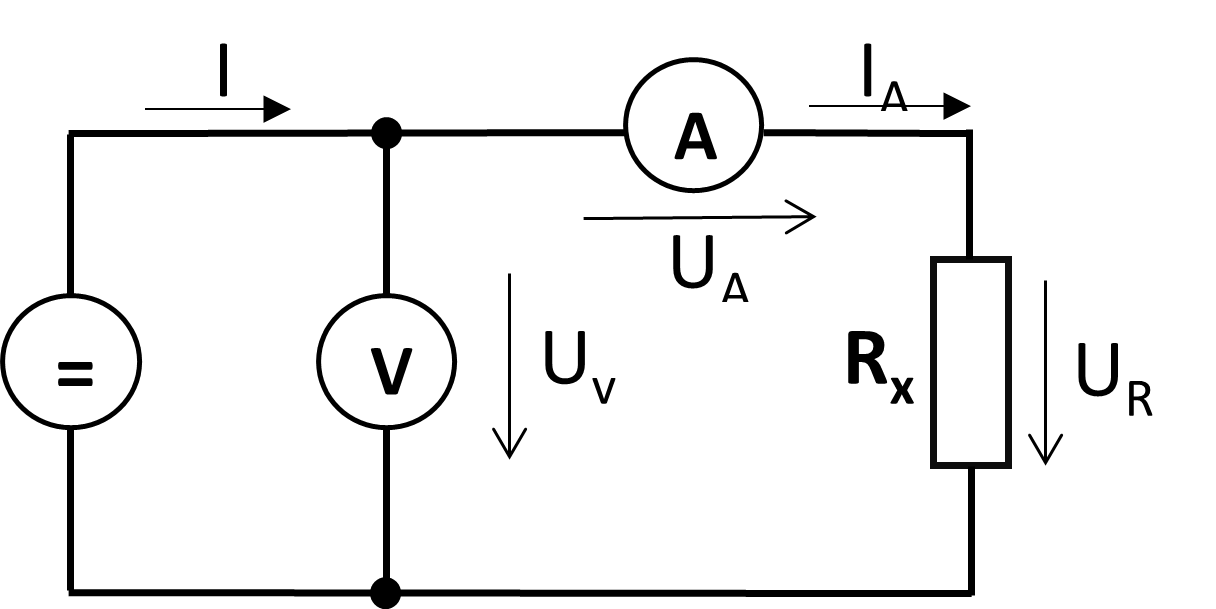
\includegraphics[width=0.3\textwidth]{schema1.png}
    \caption{Schéma uspořádání VA pro měření odporu Ohmovou metodou}
\end{figure}

\subsubsection{Uspořádání AV}

Ampérmetr měří součet elektrických proudů protékaných měřeným odporem i voltmetrem. 
Volíme pro měření menších odporů, kde je měřeňý odpor mnohem menší než vnitřní odpor voltmetru.

\begin{figure}[H]
    \centering
    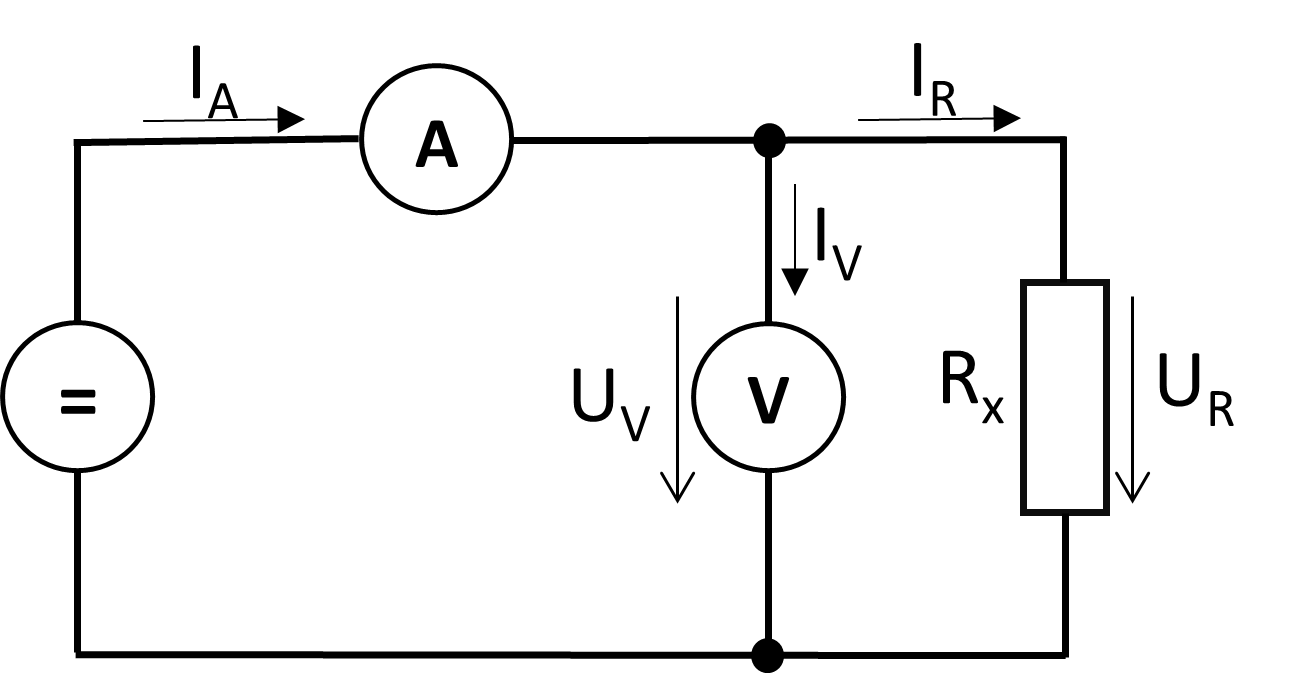
\includegraphics[width=0.3\textwidth]{schema2.png}
    \caption{Schéma uspořádání AV pro měření odporu Ohmovou metodou}
\end{figure}

\subsection{Substituční metoda}

Jedná se o zvláštní případ srovnávací metody.
Tato metoda postavena na porovnávání velikosti měřeného odporu s odporem známé velikosti (etalonem).

\begin{figure}[H]
    \centering
    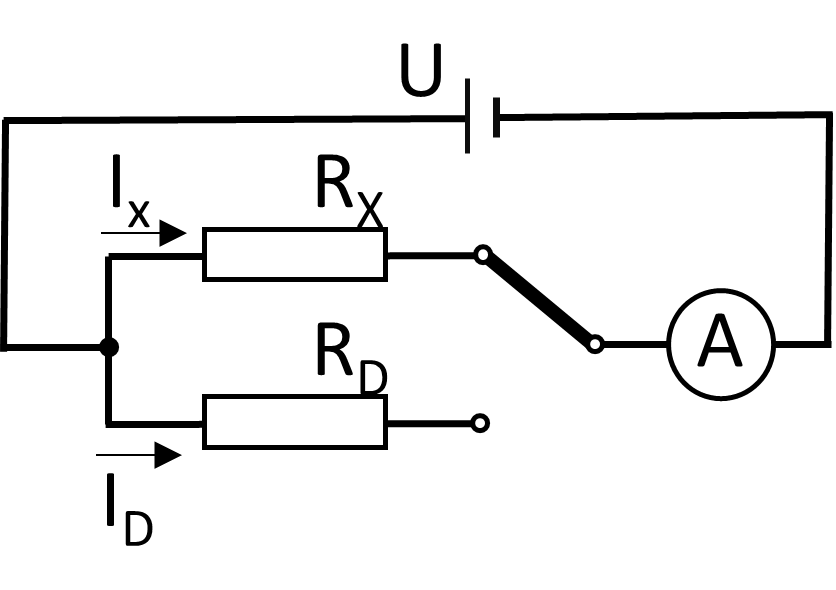
\includegraphics[width=0.3\textwidth]{schema3.png}
    \caption{Schéma zapojení pro měření odporu substituční metodou}
\end{figure}

\subsection{Převodník odpor-napětí s operačním zesilovačem}

Tato metoda využív měření odporů s využitím číslicového voltmetru, ke kterému přidáme převodník, jehož výstupní napětí bude úměrné velkosti připojeného měřeného odporu.
K tomuto účelu lze využít operační zesilovač, do jeho zpětné vazby se zapojí měřený odpor podle schématu.

\begin{figure}[H]
    \centering
    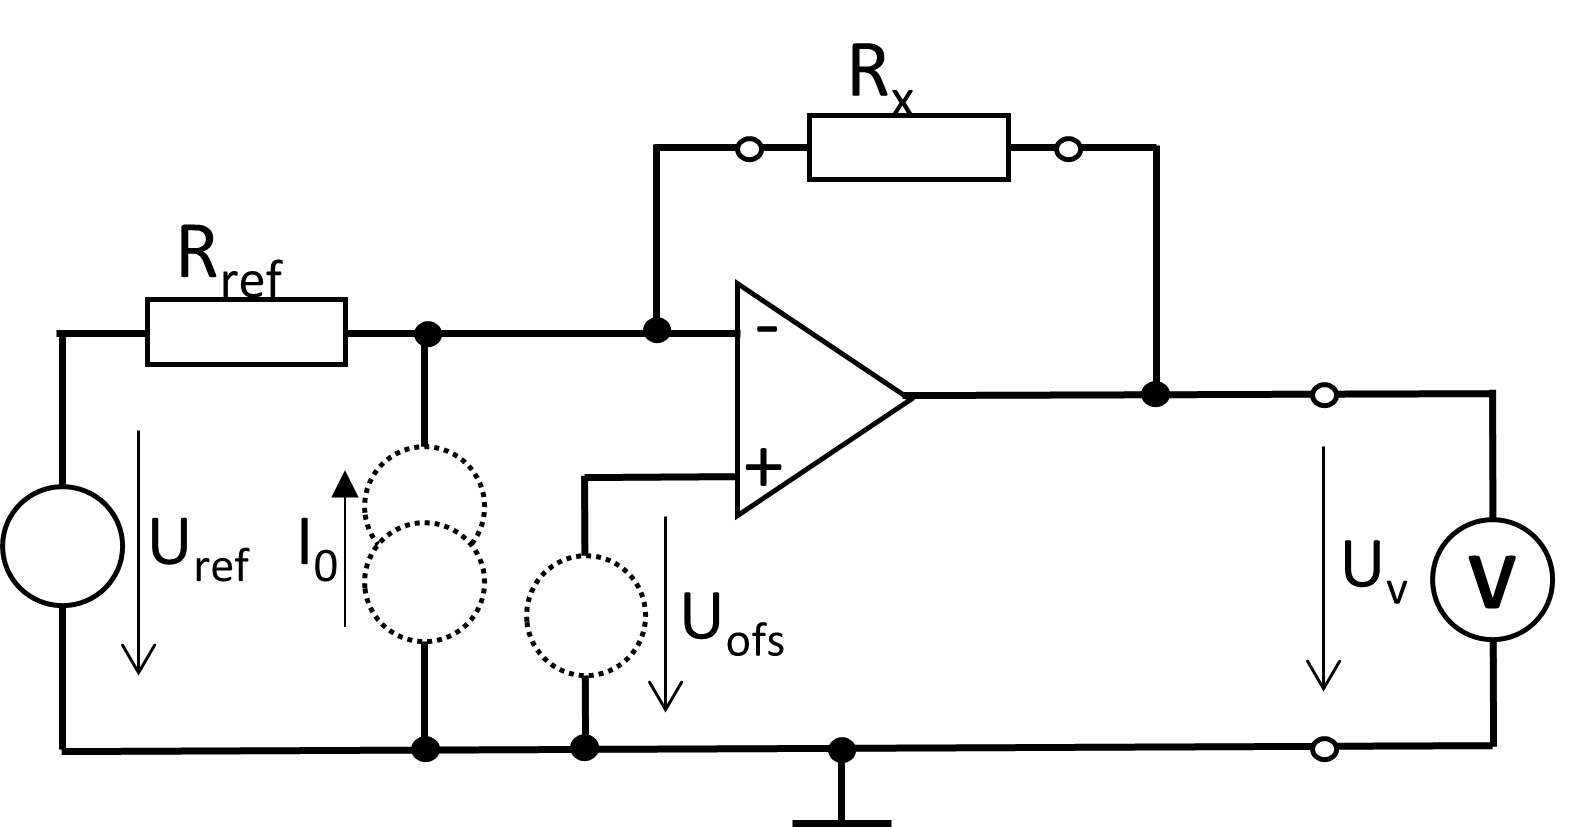
\includegraphics[width=0.5\textwidth]{schema4.png}
    \caption{Schéma zapojení jednoduchého převodníku pro měření odporu}
\end{figure}

\pagebreak

\section{Výsledky měření}

\subsection{Tabulky}

\begin{table}[H]
    \catcode`\-=12
    \centering
    \caption{Naměřené a vypočtené hodnoty pro Ohmovu metodu VA}
    \begin{tabular}{lcccccccccccc}
        \toprule
        \multirow{2}{*}{} & \multicolumn{3}{c}{$I_A$} & \multicolumn{3}{c}{$U_V$} & $R'_{X_{VA}}$ & $R_A$ & $\Delta_{R_{X_{VA}}}$ & $\delta_{R_{X_{VA}}}$ & $R_{X_{VA}}$ & $\tilde{U}_{R_{X_{VA}}}$ \\
        \cmidrule(rl){2-4}
        \cmidrule(rl){5-7}
        \cmidrule(rl){8-8}
        \cmidrule(rl){9-9}
        \cmidrule(rl){10-10}
        \cmidrule(rl){11-11}
        \cmidrule(rl){12-12}
        \cmidrule(rl){13-13}
        & $\alpha_A$   & $k_A$       & mA     & $\alpha_V$    & $k_V$       & V     & $\Omega$         & $\Omega$    & $\Omega$               & \%              & $\Omega$        & \%          \\
        \midrule
        $R_1$                & 109  & 120/120  & 109    & 75    & 2,4/120  & 1,5   & 13,7615   & 4,1  & 4,1             & 42,44           & 9,6615   & 1,597       \\
        $R_2$                & 111  & 6/120    & 5,55   & 75    & 2,4/120  & 1,5   & 270,27    & 72   & 72              & 36,31           & 198,27   & 1,520       \\
        $R_3$                & 111  & 120/120  & 111    & 76    & 12/120   & 7,6   & 68,468    & 4,1  & 4,1             & 6,370           & 64,368   & 1,175       \\
        $R_4$                & 108  & 2,4/120  & 2,16   & 102   & 12/120   & 10,2  & 4722,2    & 156  & 156             & 3,416           & 4566,2   & 0,966       \\
        $R_5$                & 77   & 0,6/120  & 0,385  & 115   & 12/120   & 11,5  & 29870     & 250  & 250             & 0,844           & 29620    & 1,092      \\
        \bottomrule
        \multicolumn{12}{l}{$\delta_{TP_V} = 0,5\%;\ \delta_{TP_A} = 0,5\%$}
    \end{tabular}
\end{table}

\begin{table}[H]
    \catcode`\-=12
    \centering
    \caption{Naměřené a vypočtené hodnoty pro Ohmovu metodu AV}
    \begin{tabular}{lcccccccccccc}
        \toprule
        \multirow{2}{*}{} & \multicolumn{3}{c}{$I_A$} & \multicolumn{3}{c}{$U_V$} & $R'_{X_{AV}}$ & $R_V$ & $\Delta_{R_{X_{AV}}}$ & $\delta_{R_{X_{AV}}}$ & $R_{X_{AV}}$ & $\tilde{U}_{R_{X_{AV}}}$ \\
        \cmidrule(rl){2-4}
        \cmidrule(rl){5-7}
        \cmidrule(rl){8-8}
        \cmidrule(rl){9-9}
        \cmidrule(rl){10-10}
        \cmidrule(rl){11-11}
        \cmidrule(rl){12-12}
        \cmidrule(rl){13-13}
        & $\alpha_A$   & $k_A$       & mA     & $\alpha_V$    & $k_V$       & V     & $\Omega$         & $\Omega$    & $\Omega$               & \%              & $\Omega$        & \%          \\
        \midrule
        $R_1$                & 108   & 120/120  & 108   & 108   & 1,2/120  & 1,08  & 10,000    & 1200  & -0,0840         & -0,833          & 10,084   & 0,915       \\
        $R_2$                & 103   & 120/120  & 103   & 111   & 24/120   & 22,2  & 215,53    & 24000 & -1,9532         & -0,898          & 217,49   & 0,926       \\
        $R_3$                & 115   & 120/120  & 115   & 73    & 12/120   & 7,3   & 63,478    & 12000 & -0,3376         & -0,529          & 63,816   & 1,130       \\
        $R_4$                & 109   & 6/120    & 5,45  & 105   & 24/120   & 21    & 3853,2    & 24000 & -736,95         & -16,06          & 4590,2   & 1,091       \\
        $R_5$                & 69    & 2,4/120  & 1,38  & 117   & 12/120   & 11,7  & 8478,3    & 12000 & -20411          & -70,65          & 28889    & 3,972      \\
        \bottomrule
        \multicolumn{12}{l}{$R_V = 1000 \Omega \slash V;\ \delta_{TP_V} = 0,5\%;\ \delta_{TP_A} = 0,5\%$}
    \end{tabular}
\end{table}

\begin{table}[H]
    \catcode`\-=12
    \centering
    \caption{Naměřené a vypočtené hodnoty pro měření převodníkem}
    \begin{tabular}{lcccccc}
        \toprule
        \multirow{2}{*}{} & $R_{ref}$ & \multicolumn{2}{c}{$U_V$} & $R_X$   & $\tilde{U}_{R_X}$ \\
        \cmidrule(rl){2-2} 
        \cmidrule(rl){3-4}
        \cmidrule(rl){5-5}
        \cmidrule(rl){6-6}
        & $\Omega$      & $X_R$         & V           & $\Omega$      & \%      \\ 
        \midrule
        $R_1$                & 500    & 0,1        & -0,10       & 10,09  & 0,141   \\ 
        $R_2$                & 500    & 10         & -2,19       & 219,03 & 0,136   \\ 
        $R_3$                & 500    & 0,1        & -0,10       & 9,919  & 0,141   \\ 
        $R_4$                & 5000   & 10         & -4,67       & 4667   & 0,132   \\ 
        $R_5$                & 50000  & 10         & -3,03       & 30312  & 0,134   \\ 
        \bottomrule
        \multicolumn{6}{l}{$U_{ref} = 5V;\ R_{ref} = 500 \Omega \text{ až } 5 M \Omega$}
    \end{tabular}
\end{table}

\begin{table}[H]
    \catcode`\-=12
    \centering
    \caption{Naměřené hodnoty pro substituční metodu}
    \begin{tabular}{lccc}
        \toprule
        \multirow{2}{*}{} & $I$   & $R_X = R_D$ & $\tilde{U}_{R_X}$                \\
        \cmidrule(rl){2-2}
        \cmidrule(rl){3-3}
        \cmidrule(rl){4-4}
                                     & mA  & $\Omega$           & \%                     \\
        \midrule
        $R_1$                           & 106 & 9,1         & \multirow{5}{*}{0,115} \\
        $R_2$                           & 103 & 218         &                        \\
        $R_3$                           & 101 & 57,2        &                        \\
        $R_4$                           & 5,0   & 4680        &                        \\
        $R_5$                           & 0,5 & 30400       &                       \\
        \bottomrule
        \multicolumn{4}{l}{$\delta_{R_D} = 0,1\%$}
    \end{tabular}
\end{table}

\begin{table}[H]
    \catcode`\-=12
    \centering
    \caption{Srovnání výsledků jednotlivých metod}
    \begin{tabular}{lcccccccccc}
        \toprule
        \multirow{2}{*}{}    & $R_1$     & $\tilde{U}_{R_1}$ & $R_2$      & $\tilde{U}_{R_1}$ & $R_3$     & $\tilde{U}_{R_1}$ & $R_4$       & $\tilde{U}_{R_1}$ & $R_5$    & $\tilde{U}_{R_1}$ \\
        \cmidrule(rl){2-3}
        \cmidrule(rl){4-5}
        \cmidrule(rl){6-7}
        \cmidrule(rl){8-9}
        \cmidrule(rl){10-11}
                            & $\Omega$      & \%    & $\Omega$       & \%    & $\Omega$      & \%    & $\Omega$        & \%    & $\Omega$     & \%    \\
        \midrule
        Ohmova   metoda VA   & 9,6615 & 1,597 & 198,27 & 1,520 & 64,368 & 1,175 & 4566 & 0,966 & 29620 & 1,092 \\
        Ohmova   metoda AV   & 10,084 & 0,915 & 217,49  & 0,926 & 63,816 & 1,130 & 4590   & 1,091 & 28889 & 3,972 \\
        Převodník   s OZ     & 10,09  & 0,141 & 219,03  & 0,136 & 9,919  & 0,141 & 4667     & 0,132 & 30312 & 0,134 \\
        Substituční   metoda & 9,10    & 0,115 & 218,00     & 0,115 & 57,2   & 0,115 & 4680     & 0,115 & 30400 & 0,115 \\
        \bottomrule
    \end{tabular}
\end{table}

\subsection{Příklady výpočtu}

\subsubsection{Ohmova metoda - uspořádání VA}

\begin{enumerate}
    \item Odpor vypočítaný z údajů přístrojů
    \begin{multline*}
        R'_{X_{VA}} = \textcolor{teal}{\frac{U_V}{I_A}} = \frac{1,3V}{109 \cdot 10^{-3}A} = \underline{\underline{13,76\ \Omega}} \hfill
    \end{multline*}
    \item Skutečná hodnota měřeného odporu
    \begin{multline*}
        R_{X_{VA}} = \textcolor{teal}{\frac{U_V}{I_A} - R_A} = \frac{1,3V}{109 \cdot 10^{-3}A} - 4,1 \Omega = \underline{\underline{9,661\ \Omega}} \hfill
    \end{multline*}
    \item Absolutní odchylka metody zapojení VA
    \begin{multline*}
        \Delta_{R_{X_{VA}}} = \textcolor{teal}{R'_{X_{VA}} - R_{X_{VA}}} = 13,76 \Omega - 9,661 \Omega = \underline{\underline{4,1\ \Omega}} \hfill
    \end{multline*}
    \item Relativní odchylka metody
    \begin{multline*}
        \delta_{R_{X_{VA}}} = \textcolor{teal}{\frac{R_A}{R_{X_{VA}}} \cdot 100\%} = \frac{4,1 \Omega}{9,661 \Omega} \cdot 100\% = \underline{\underline{42,43\ \%}} \hfill
    \end{multline*}
    \item Standardní přístrojová nejistota AMP (typu B)
    \begin{multline*}
        u_{BU} = \textcolor{teal}{\frac{\delta_{TP} \cdot X_R}{100 \% \cdot \chi}} = \frac{\delta_{TP_V} \cdot U_R}{100 \% \cdot \sqrt{3}} = \frac{0,5\% \cdot 2,4V}{100 \% \cdot \sqrt{3}} = 6,928 \cdot 10^{-3} V = \underline{\underline{6,928\ mV}} \hfill
    \end{multline*}
    \begin{multline*}
        u_{BI} = \frac{\delta_{TP_A} \cdot I_R}{100 \% \cdot \sqrt{3}} = \frac{0,5\% \cdot 120 \cdot 10^{-3}A}{100 \% \cdot \sqrt{3}} = 346,4 \cdot 10^{-6} A = \underline{\underline{346,4\ \mu A}} \hfill
    \end{multline*}
    \item Standardní nejistota výsledku
    \begin{multline*}
        u_{R_{X_{VA}}} = \textcolor{teal}{\sqrt{\left(\frac{1}{I_A} \cdot u_{BU}\right)^2 + \left(\frac{U_V}{I_A^2} \cdot u_{BI}\right)^2}} =  \hfill \\
        = \sqrt{\left(\frac{1}{109 \cdot 10^{-3}A} \cdot 6,928 \cdot 10^{-3} V\right)^2 + \left(\frac{1,5V}{(109 \cdot 10^{-3}A)^2} \cdot 346,4 \cdot 10^{-6} A\right)^2} = 77,15 \cdot 10^{-3} \Omega = \underline{\underline{77,15\ m \Omega}} \hfill
    \end{multline*}
    \item Relativní rozšířená nejistota
    \begin{multline*}
        \tilde{U}_{R_{X_{VA}}} = \frac{u_{R_{X_{VA}}} \cdot k_r}{R_{X_{VA}}} \cdot 100\% = \frac{77,15 \cdot 10^{-3} \Omega \cdot 2}{9,661 \Omega} \cdot 100\% = \underline{\underline{1,597\ \%}} \hfill
    \end{multline*}
\end{enumerate}

\subsubsection{Ohmova metoda - uspořádání AV}

\begin{enumerate}
    \item Odpor vypočítaný z údajů přístrojů
    \begin{multline*}
        R'_{X_{AV}} = \textcolor{teal}{\frac{U_V}{I_A}} = \frac{1,08V}{108 \cdot 10^{-3}A} = \underline{\underline{10\ \Omega}} \hfill
    \end{multline*}
    \item Skutečná hodnota měřeného odporu
    \begin{multline*}
        R_{X_{AV}} = \textcolor{teal}{\frac{U_V}{I_A - \frac{U_V}{R_V}}} = \frac{1,08V}{108 \cdot 10^{-3}A - \frac{1,08V}{1200 \Omega}} = \underline{\underline{10,08\ \Omega}} \hfill
    \end{multline*}
    \item Absolutní odchylka metody zapojení AV
    \begin{multline*}
        \Delta_{R_{X_{AV}}} = \textcolor{teal}{R'_{X_{AV}} - R_{X_{AV}}} = 10 \Omega - 10,08 \Omega = \underline{\underline{-0,08\ \Omega}} \hfill
    \end{multline*}
    \item Relativní odchylka metody
    \begin{multline*}
        \delta_{R_{X_{AV}}} = \textcolor{teal}{\frac{\Delta_{R_{X_{AV}}}}{R_{X_{AV}}} \cdot 100\%} = \frac{0,08 \Omega}{10,08 \Omega} \cdot 100\% = \underline{\underline{-0,833\ \%}} \hfill
    \end{multline*}
    \item Standardní nejistota výsledku
    \begin{multline*}
        u_{R_{X_{AV}}} = \textcolor{teal}{\sqrt{\left(\frac{I_A \cdot u_{BU}}{\left(I_A - \frac{U_V}{R_V}\right)^2}\right)^2 + \left(\frac{U_V \cdot u_{BI}}{\left(I_A - \frac{U_V}{R_V}\right)^2}\right)^2}} = \hfill \\
        = \sqrt{\left(\frac{108 \cdot 10^{-3}A \cdot 3,464 \cdot 10^{-3}V}{\left(108 \cdot 10^{-3}A - \frac{1,08V}{1200 \Omega}\right)^2}\right)^2 + \left(\frac{1,08V \cdot 346,4 \cdot 10^{-6} A}{\left(108 \cdot 10^{-3}A - \frac{1,08V}{1200 \Omega}\right)^2}\right)^2} = 44,12 \cdot 10^{-3} \Omega = \underline{\underline{44,12\ \Omega}} \hfill
    \end{multline*}
    \item Relativní rozšířená nejistota
    \begin{multline*}
        \tilde{U}_{R_{X_{AV}}} = \frac{u_{R_{X_{AV}}} \cdot k_r}{R_{X_{AV}}} \cdot 100\% = \frac{44,12 \cdot 10^{-3} \Omega \cdot 2}{10,08 \Omega} \cdot 100\% = \underline{\underline{0,91\ \%}} \hfill
    \end{multline*}
\end{enumerate}

\subsubsection{Převodník odpor-napětí s operačním zesilovačem}

\begin{enumerate}
    \item Velikost měřeného odporu
    \begin{multline*}
        R_X = \textcolor{teal}{- \frac{R_{ref}}{U_{ref}} \cdot U_V} = - \frac{500 \Omega}{5V} \cdot (- 100,942 \cdot 10^{-3}V) = \underline{\underline{10,09\ \Omega}} \hfill
    \end{multline*}
    \item Standardní nejistota zdroje referenčního napětí
    \begin{multline*}
        u_{BU_{ref}} = \textcolor{teal}{\frac{\delta_{U_{ref}} \cdot U_{ref}}{100\% \cdot \chi}} = \frac{0,05\% \cdot 5V}{100\% \cdot \sqrt{3}} = 1,443 \cdot 10^{-3}V = \underline{\underline{1,443\ mV}} \hfill
    \end{multline*}
    \item Standardní nejistota referenčního odporu
    \begin{multline*}
        u_{BR_{ref}} = \textcolor{teal}{\frac{\delta_{U_{ref}} \cdot U_{ref}}{100\% \cdot \chi}} = \frac{0,1\% \cdot 500 \Omega}{100\% \cdot \sqrt{3}} = 288,6 \cdot 10^{-3} \Omega = \underline{\underline{288,6\ m\Omega}} \hfill
    \end{multline*}
    \item Standardní nejistota vlivu napěťové nesymetrie
    \begin{multline*}
        u_{BU_{ofs}} = \textcolor{teal}{\frac{U_{ofs}}{\sqrt{3}}} = \frac{40 \cdot 10^{-6} V}{\sqrt{3}} = 23,09 \cdot 10^{-6} V = \underline{\underline{23,09\ \mu V}} \hfill
    \end{multline*}
    \item Standardní přístrojové nejistota voltmetru
    \begin{multline*}
        u_{BU} = \textcolor{teal}{\frac{\left|\delta_M \cdot X_M\right| + \left|\delta_R \cdot X_R\right|}{100 \% \cdot \chi}} = \frac{\left|0,018\% \cdot (- 100,942 \cdot 10^{-3}V)\right| + \left|0,008\% \cdot 100 \cdot 10^{-3}V\right|}{100 \% \cdot \sqrt{3}} = \hfill \\
        = 15,10 \cdot 10^{-6} V = \underline{\underline{15,1\ \mu V}} \hfill
    \end{multline*}
    \item Standardní nejistota výsledku měření odporu
    \begin{multline*}
        u_{R_X} = \textcolor{teal}{\sqrt{\left(\frac{-R_{ref}}{U_{ref}} u_{BU}\right)^2 + \left(\frac{-R_{ref} \cdot U_V}{U_{ref}^2} u_{BU_{ref}}\right)^2 + \left(\frac{-U_V}{U_{ref}} u_{BR_{ref}}\right)^2 + \left(\frac{R_{ref} \left(U_{ref} - U_V\right)}{U_{ref}^2} u_{BU_{ofs}}\right)^2}} = \hfill \\
        = \sqrt{\left(\frac{-500 \Omega}{5V} \cdot 15,10 \cdot 10^{-6} V\right)^2 + \left(\frac{-500 \Omega \cdot (- 100,942 \cdot 10^{-3}V)}{(5V)^2} \cdot 1,443 \cdot 10^{-3}V\right)^2 + } \hfill \\
        \overline{+ \left(\frac{-(- 100,942 \cdot 10^{-3}V)}{5V} \cdot 288,6 \cdot 10^{-3} \Omega\right)^2 + \left(\frac{500 \Omega \cdot \left(5V - (- 100,942 \cdot 10^{-3}V)\right)}{(5V)^2} \cdot 23,09 \cdot 10^{-6} V\right)^2} = \hfill \\
        = 7,091 \cdot 10^{-3} \Omega = \underline{\underline{7,091\ m\Omega}} \hfill
    \end{multline*}
    \item Relativní rozšířená nejistota
    \begin{multline*}
        \tilde{U}_{R_X} = \textcolor{teal}{k_r \cdot \frac{u_{R_X}}{R_X} \cdot 100 \%} = 2 \cdot \frac{7,091 \cdot 10^{-3} \Omega}{10,09 \Omega} \cdot 100 \% = \underline{\underline{0,134\ \%}} \hfill
    \end{multline*}
\end{enumerate}

\subsubsection{Substituční metoda}

\begin{enumerate}
    \item Relativní rozšířená nejistota
    \begin{multline*}
        \tilde{U}_{R_X} = \textcolor{teal}{k_r \cdot \frac{\delta_{R_D}}{\chi}} = 2 \cdot \frac{0,1\%}{\sqrt{3}} = \underline{\underline{0,115\ \%}} \hfill
    \end{multline*}
\end{enumerate}

\section{Seznam použitých přístrojů}

\subsection{Ohmova metoda}

\begin{itemize}
    \item Analogový laboratorní miliampérmetr Metra, v.č. 101786
    \item Analogový laboratorní voltmetr Metra, v.č. 4674001
    \item Laboratorní přípravek Měření odporů středních hodnot
    \item Laboratorní zdroj jednosměrného napětí AxioMet - AX-3005DLS, v.č. 713063
\end{itemize}

\subsection{Substituční metoda a metoda s převodníkem}

\begin{itemize}
    \item Analogový laboratorní miliampérmetr Metra, v.č. 976896
    \item Odporová dekáda Metra XL6, v.č. 7910443
    \item Laboratorní přípravek s přepínačem
    \item Laboratorní zdroj jednosměrného napětí AxioMet - AX-3005DLS, v.č. 713062
    \item Laboratorní číslicový multimetr Keysight 34450A, v.č MY58180037
    \item Převodník odpor-napětí
\end{itemize}

\section{Závěr}

Naší úlohou bylo určit hodnoty předložených neznámých odporů Ohmovou metodou, substituční metodou a metodou s převodníkem.
Hodnoty odporů určené Ohmovou metodou jsou uvedeny v tabulce číslo 1 spolu s ostatními vypočtenými hodnotami.
Experimentálně jsme si ověřili, že uspořádání VA Ohmovy metody je vhodné pro měření řádově velkých odporů.
Naopak, uspořádání AV Ohmovy (výsledky v tabulce číslo 2) metody je vhodné pro měření řádově malých odporů.

Měřením provedeném substituční metodou jsme empiricky zjistili, že má konstantní nejistotu.
Zdrojem této konstantní nejistoty je použitá odporové dekáda.

Při měření neznámých odporů metodou s převodníkem je patrné, že hodnoty relativních nejistot mezi jednotlivými měřeními liší jen o malou odchylku.
Zdroj tohoto jevu je stálost referenčního napětí a referenčního odporu použitého převodníku.
Je též patrné, že tato metoda vykazuje nejmenší relativní nejistoty ve srovnání s ostatními použitými metodami.

Naměřené hodnoty odporu $R_3$ se mezi použitými metodami poměrně liší.
Jedním z důvodů pro tento jev může být, že se nejedná o rezistor, ale jiný prvek s nelineární odporovou charakteristikou.

Chyby v měřeních jsou způsobeny systematickými odchylkami z použitých metod měření, nejistotami použitých přístrojů ale také systematickou odchylkou zavedenou námi během měření.

\end{document}